\section{A Reminder on Probability Theory}
\label{appendix:prob_theory_reminder}
We present a brief overview of basic concepts from probability theory. This section was partially taken from \citep{lipman2024flow}.
\subsection{Random vectors}

Consider data in the $d$-dimensional Euclidean space $x=(x^1,\ldots,x^d)\in \Real^d$ with the standard Euclidean inner product $\ip{x,y}=\sum_{i=1}^d x^i y^i$ and norm $\norm{x}=\sqrt{\ip{x,x}}$.
%
We will consider random variables (RVs) $X\in\R^d$ with continuous probability density function (PDF), defined as a \emph{continuous} function $p_X:\Real^d\too \Real_{\geq 0}$ providing event $A$ with probability
%
\begin{equation}
    \sP(X\in A) = \int_A p_X(x) \dd x,
\end{equation}
%
where $\int p_X(x)\dd x = 1$.
%
By convention, we omit the integration interval when integrating over the whole space ($\int \equiv \int_{\Real^d}$).
%
To keep notation concise, we will refer to the PDF $p_{X_t}$ of RV $X_t$ as simply $p_t$.
%
We will use the notation $X \sim p$ or $X \sim p(X)$ to indicate that $X$ is distributed according to $p$.
%
One common PDF in generative modeling is the $d$-dimensional isotropic Gaussian:
%
\begin{equation}\label{e:gaussian}
  \gN(x;\mu,\sigma^2 I) = (2\pi\sigma^2)^{-\frac{d}{2}}\exp\left(-\frac{\norm{x-\mu}_2^2}{2\sigma^2}\right),
\end{equation}
%
where $\mu\in \Real^d$ and $\sigma \in \Real_{>0}$ stand for the mean and the standard deviation of the distribution, respectively.

%

The expectation of a RV is the constant vector closest to $X$ in the least-squares sense:
%
\begin{equation}\label{e:E}
    \E\brac{X}=\argmin_{z\in\Real^d} \int \norm{x-z}^2 p_X(x)\dd x = \int x p_X(x)\dd x. % \qquad \metatriangleright\, \highlight{\text{expectation of a random variable}} 
\end{equation}
%
One useful tool to compute the expectation of \emph{functions of RVs} is the \emph{law of the unconscious statistician}:
%
% which is essentially a change of variables in integration theorem, reads:
%
\begin{equation}\label{e:law_of_uncon_stat}
    \E \brac{f(X)} = \int f(x) p_X(x) \dd x. % \qquad \metatriangleright\,\highlight{\text{Law of the Unconscious Statistician}}
\end{equation}
%
When necessary, we will indicate the random variables under expectation as $\E_{X} f(X)$.

%

% \yl{weak convergence of random variables $p_t\too p$ as $t\too 1$ is defined by $\E f(X_t) \too \E f(X)$ (standard convergence of scalar series) as $t\too 1$ for all continuous bounded $f$. }

\subsection{Conditional densities and expectations} \label{sec:conditional_densities_and_expectations}
%
\begin{wrapfigure}{r}{0.25\textwidth}
  \vspace{-40pt}
  \begin{center}
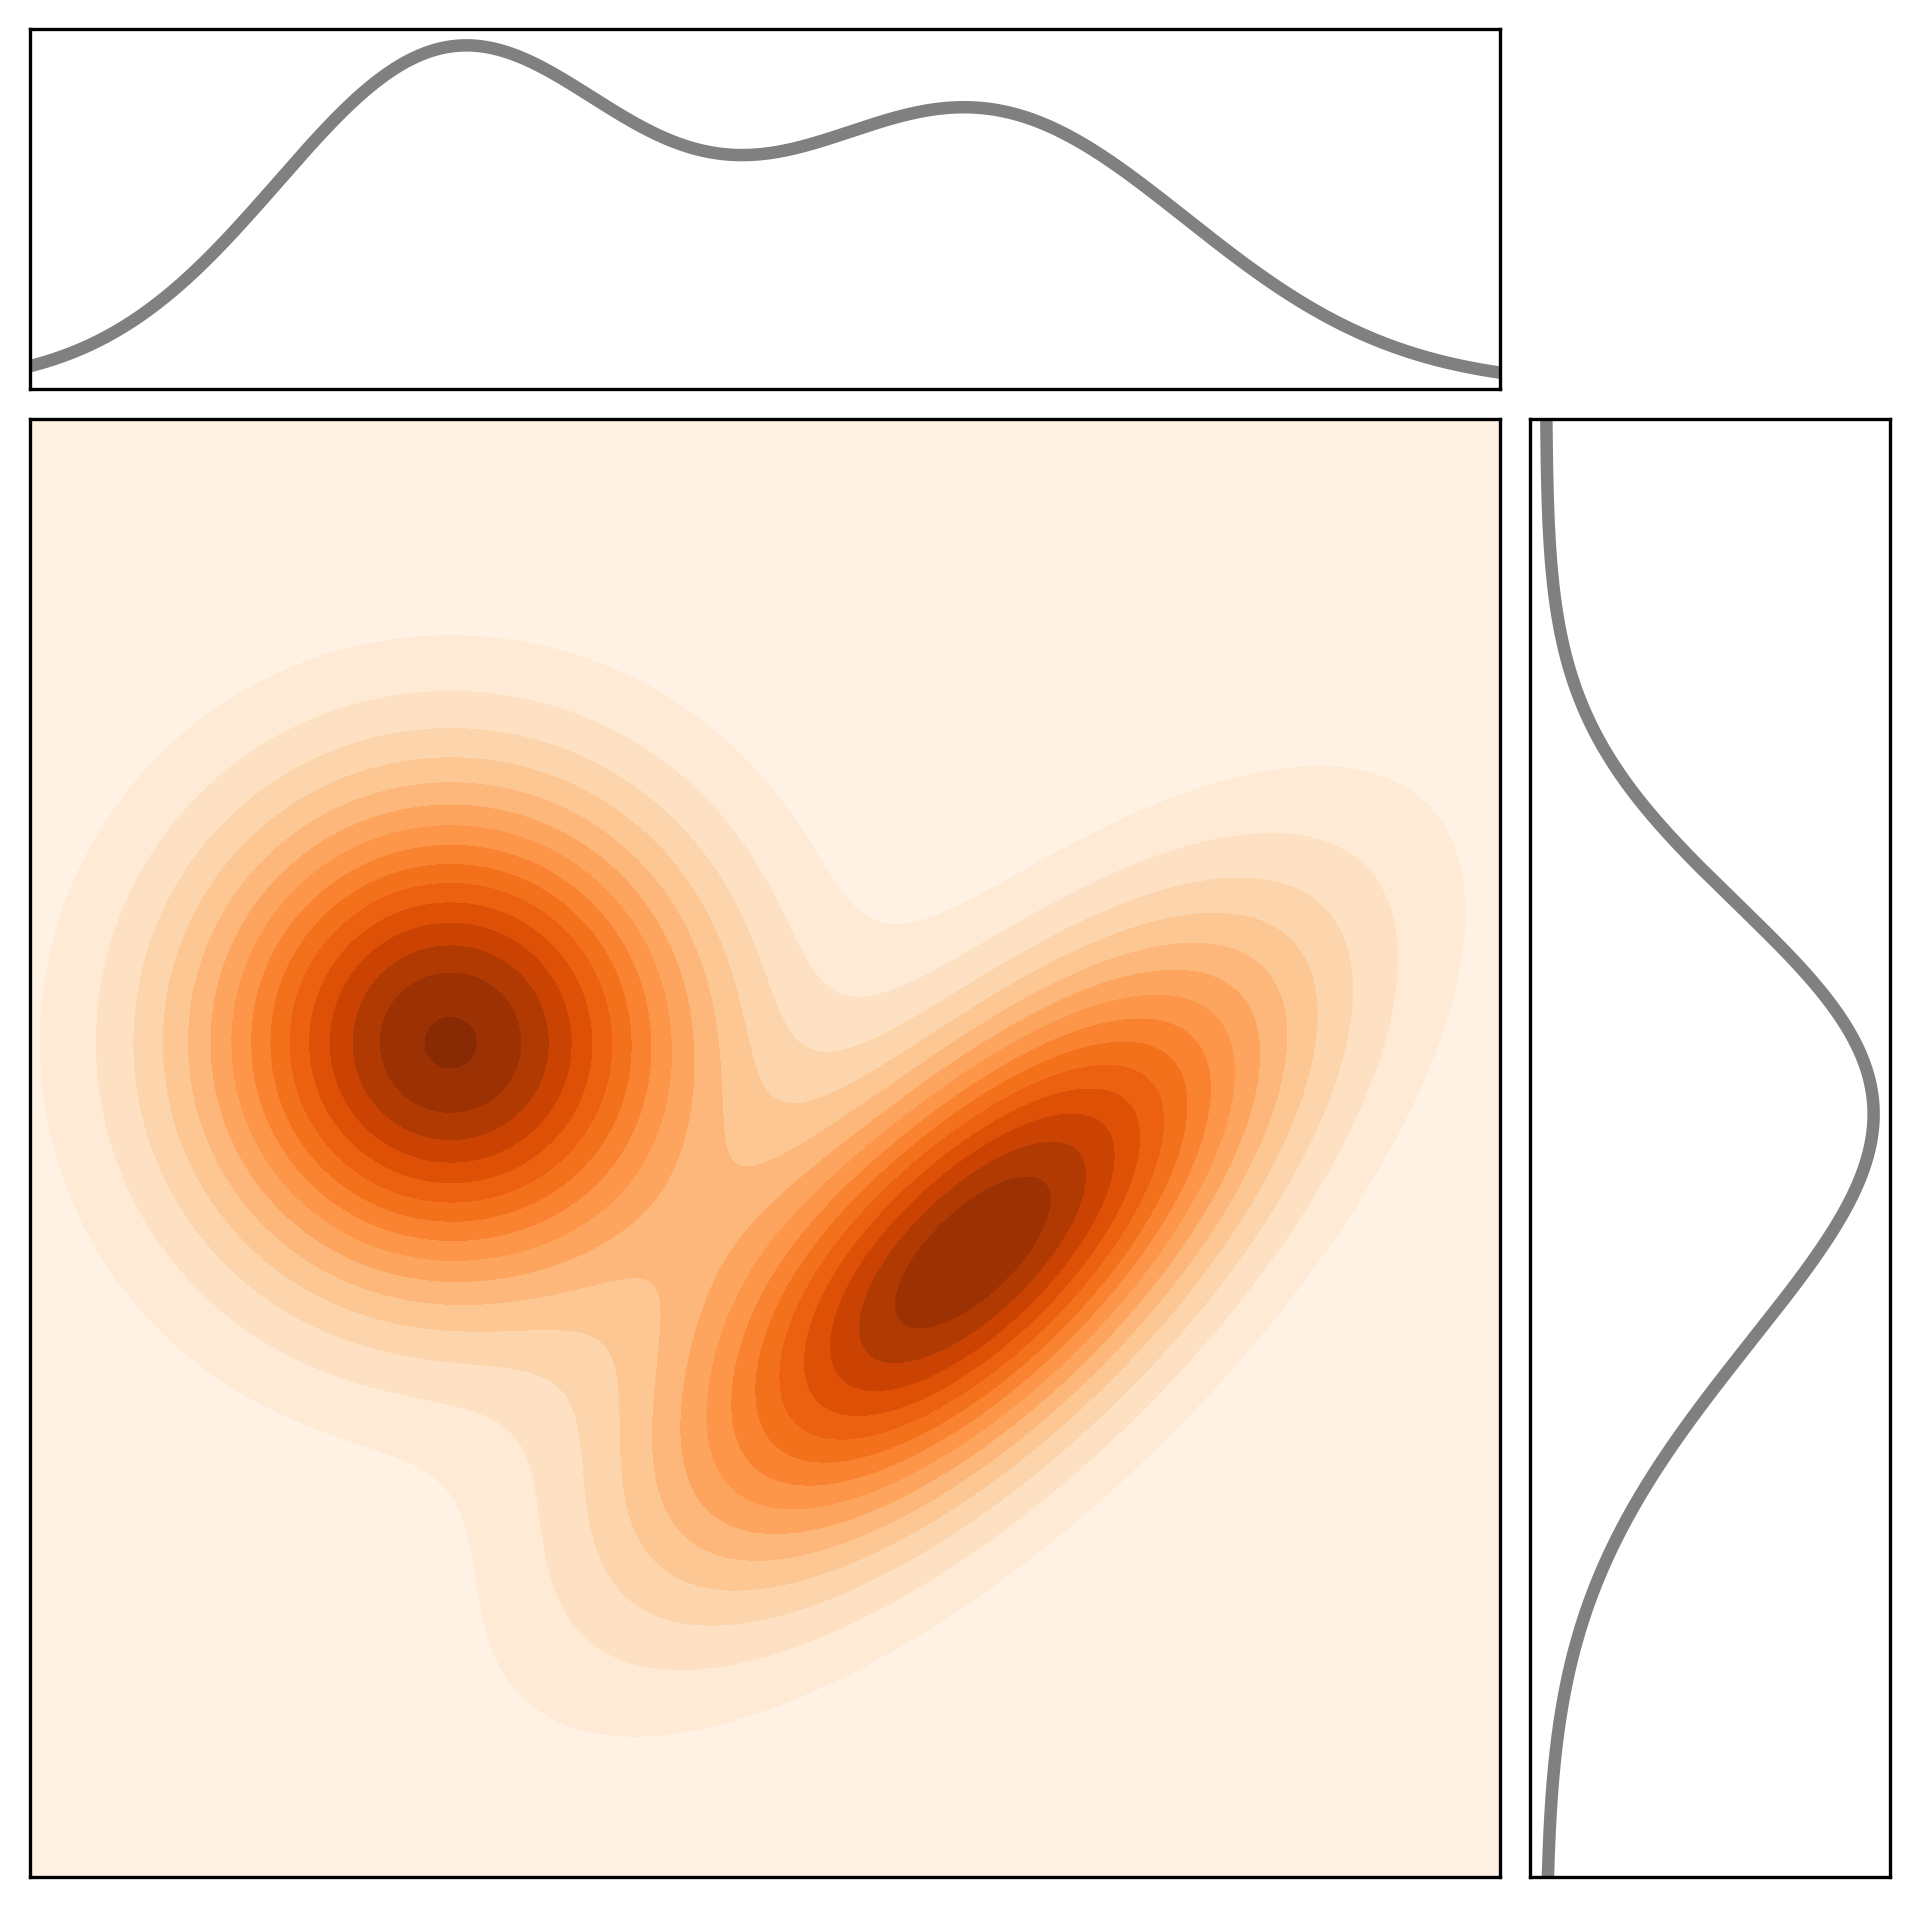
\includegraphics[width=0.25\textwidth]{figures/joints.png}
  \end{center}
  \caption{Joint PDF $p_{X,Y}$ (in shades) and its marginals $p_X$ and $p_Y$ (in black lines). Figure from \citep{lipman2024flow}}.
  \label{fig:joint}
\end{wrapfigure}

Given two random variables $X,Y\in \Real^d$, their joint PDF $p_{X,Y}(x,y)$ has marginals 
%
\begin{equation}\label{e:marginals}
 \int p_{X,Y}(x,y)\dd y = p_X(x) \text{ and } \int p_{X,Y}(x,y)\dd x = p_Y(y). 
\end{equation}
See \cref{fig:joint} for an illustration of the joint PDF of two RVs in $\Real$ ($d=1$). 
%
% $X\sim p$ and $Y\sim q$, their \emph{joint distribution} $(X,Y)\sim \pi(X,Y)$ is a probability density over $\Real^d\times\Real^d$, with the marginals $\int \pi(x,y) \dd x=p(x)$ and $\int \pi(x,y)\dd x=q(y)$.
%
The \emph{conditional} PDF $p_{X|Y}$ describes the PDF of the random variable $X$ when conditioned on an event $Y=y$ with density $p_Y(y)>0$:
%
\begin{equation}\label{e:conditional}
    p_{X|Y}(x|y)\defe\frac{p_{X,Y}(x,y)}{p_Y(y)},
\end{equation} 
%
and similarly for the conditional PDF $p_{Y|X}$. Bayes' rule expresses the conditional PDF $p_{Y|X}$ with $p_{X|Y}$ by
\begin{equation}
    p_{Y|X}(y|x) = \frac{p_{X|Y}(x|y)p_Y(y)}{p_X(x)},
\end{equation}
for $p_X(x)>0$. 
%

The \emph{conditional expectation} $\E\brac{X | Y}$ is the best approximating \emph{function} $g_\star(Y)$ to $X$ in the least-squares sense: 
%
\begin{align}\nonumber
    g_\star &\defe  \argmin_{g:\Real^d\too\Real^d}\E\brac{\norm{X-g(Y)}^2} =  \argmin_{g:\Real^d\too\Real^d}\int \norm{x-g(y)}^2 p_{X,Y}(x,y)\dd x \dd y \\ \label{e:cond_E_g_star}
    &= \argmin_{g:\Real^d\too\Real^d} \int\brac{\textcolor{black}{\int \norm{x-g(y)}^2p_{X|Y}(x|y)\dd x}} p_Y(y)\dd y.
\end{align}
%
For $y\in \Real^d$ such that $p_Y(y)>0$ the conditional expectation function is therefore
%
\begin{equation}\label{e:cond_E_func}
    \E\brac{X|Y=y} \defe g_\star(y) = \int x p_{X|Y}(x|y) \dd x, %\qquad \metatriangleright\,\highlight{\text{conditional expectation (function $\Real^d\too\Real^d$)}}
\end{equation}
%
where the second equality follows from taking the minimizer of the inner brackets in \cref{e:cond_E_g_star} for $Y=y$, similarly to \cref{e:E}. 
%
Composing $g_\star$ with the random variable $Y$, we get 
%
\begin{equation}
    \E\brac{X|Y} \defe g_\star(Y), % \qquad \metatriangleright\,\highlight{\text{conditional expectation (RV $\Omega\too \Real^d$)} }
\end{equation}
%
which is a random variable in $\Real^d$.
%
Rather confusingly, both $\E\brac{X|Y=y}$ and $\E\brac{X|Y}$ are often called \emph{conditional expectation}, but these are different objects.
%
In particular, $\E\brac{X|Y=y}$ is a function $\Real^d\too\Real^d$, while $\E\brac{X|Y}$ is a random variable assuming values in $\Real^d$.
%
To disambiguate these two terms, our discussions will employ the notations introduced here. 

%

The \emph{tower property} is an useful property that helps simplify derivations involving conditional expectations of two RVs $X$ and $Y$:
%
\begin{equation}\label{e:tower}
    \E\brac{\E\brac{X|Y}} = \E\brac{X} %\qquad \metatriangleright\,\highlight{\text{tower property}}
\end{equation}
%
Because $\E\brac{X|Y}$ is a RV, itself a function of the RV $Y$, the outer expectation computes the expectation of $\E\brac{X|Y}$.
%
The tower property can be verified by using some of the definitions above: 
%
\begin{align*}
    \E\brac{\E\brac{X|Y}} &= \int \parr{\int x p_{X|Y}(x|y) \dd x} p_Y(y) \dd y \\
    &\overset{\eqref{e:conditional}}{=} \int \int x p_{X,Y}(x,y) \dd x\dd y \\
    &\overset{\eqref{e:marginals}}{=} \int x p_X(x)\dd x \\
    &= \E \brac{X}.
\end{align*}

%

Finally, consider a helpful property involving two RVs $f(X, Y)$ and $Y$, where $X$ and $Y$ are two arbitrary RVs.
%
Then, by using the Law of the Unconscious Statistician with \eqref{e:cond_E_func}, we obtain the identity
%
% %
% \begin{align*}
%     g_\star &=  \argmin_{g:\Real^d\too\Real^d} \E \brac{\norm{f(X,Y)-g(Y)}^2} \\
%     &\overset{\eqref{e:law_of_uncon_stat}}{=} \argmin_{g:\Real^d\too\Real^d} \int \brac{ \int \norm{f(x,y)-g(y)}^2 p_{X|Y}(x|y)\dd x } p_Y(y) \dd y,
% \end{align*}
% %
% which translates into the conditional expectation identity:
%
\begin{equation}\label{e:f_x_y_cond_y}
    \E\brac{f(X,Y)|Y=y} = \int f(x,y) p_{X|Y}(x|y) \dd x.
\end{equation}